% Introdução
\chapter{Introdução}

Este é o capítulo introdutório da monografia e está dividido em cinco seções. A primeira trata de contextualizar o estudo. A segunda trás a situação problema encontrada no contexto informado. Depois disso, são mostradas as possíveis soluções existentes e apresentada a proposta do estudo. Por fim, são expostos os objetivos do trabalho, os métodos e técnicas aplicadas e a motivação encontrada.

\section{Contextualização}

Como Unidade Suplementar da Universidade Federal do Rio Grande do Norte (UFRN), o Instituto Metrópole Digital (IMD) atua na formação de jovens e adultos de nível técnico, superior e pós-graduação. Suas ações integram a inclusão social e digital de estudantes do ensino básico à pós-graduação, a realização de pesquisa e inovação tecnológica e o incentivo à cultura do empreendedorismo.

Hoje o IMD encontra-se particionado em diversos setores, cada qual com seu objetivo e metodologia. Entre estes setores, há o setor de materiais, responsável pela produção de todo o material disponibilizado pelo instituto e principal interessado no desenvolvimento deste trabalho. 

Dentro do setor de materiais é possível extrair todos os fluxos que contemplam a criação de um material e, na figura a seguir, é possível entender como um dos principais fluxos funciona. \\

\vspace{5mm}
\begin{minipage}[c]{\textwidth}
    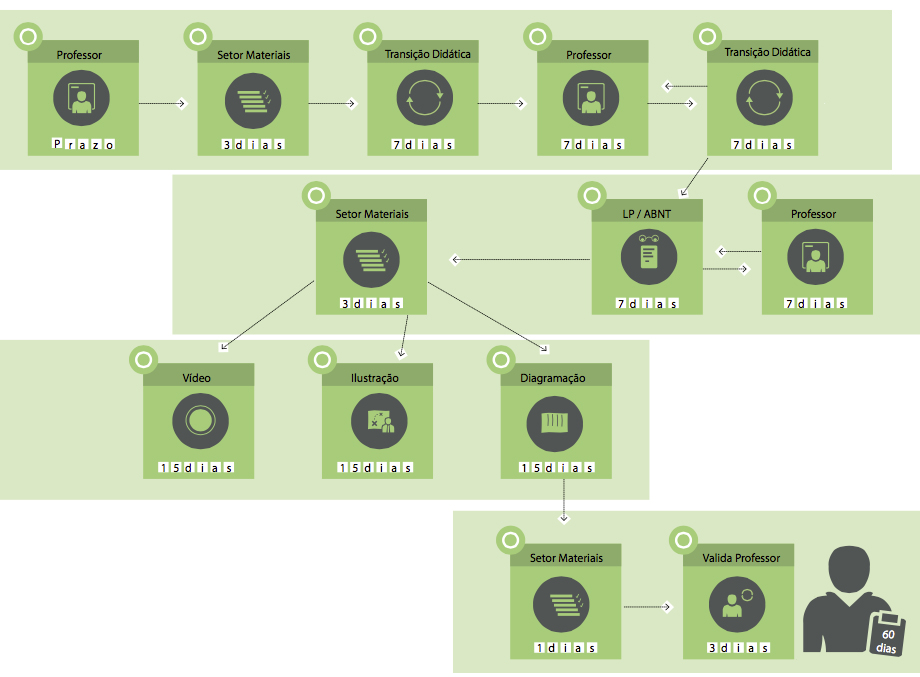
\includegraphics[width=14cm]{Imagens/FluxoMateriaisNovos.jpg}
    \captionof{figure}{Fluxo de Criação de Materiais Didáticos}
    \label{fig:fluxo_materiais_novos}
\end{minipage}
\vspace{5mm}

O fluxo da \hyperref[fig:fluxo_materiais_novos]{Figura \ref{fig:fluxo_materiais_novos}} é iniciado com o envio do arquivo pelo professor para o setor de materiais, onde será feita uma primeira análise do conteúdo do material e será repassado para a equipe pedagógica responsável pela transição didática. O material então fica alternando de etapa entre o professor e a equipe pedagógica até que a última determine a conformidade do conteúdo. Neste momento, a equipe de língua portuguesa e normas ABNT recebe o arquivo e se responsabiliza por executar revisão e melhorias juntamente com o professor, o setor de materiais recebe o resultado e, de acordo com as necessidades, solicita criação de material de vídeo, ilustração e, por último, diagramação. No momento que a equipe de diagramação termina seu trabalho, o arquivo volta ao setor de materiais para que seja feita uma nova verificação nos resultados obtidos e solicitar aprovação ao professor que iniciou o processo.

No fluxo descrito, vários papéis/equipes foram citados, cada um desses é representado na \hyperref[fig:fluxo_materiais_novos]{Figura \ref{fig:fluxo_materiais_novos}} por um bloco verde escuro e destaca um envolvido no processo, alguns deles sendo subsetores do setor de materiais e outros externos a esse. Na tabela abaixo é possível entender os seus papéis.

\begin{center}
    \begin{tabularx}{\textwidth}{ |X|X| }
    \hline
    \multicolumn{2}{|c|}{Definição de envolvidos e papéis} \\
    \hline
    Nome & Papel \\ \hline
    Professor & Elabora o material de aula/prova na sua versão inicial e participa do fluxo realizando melhorias e correções. \\ \hline
    Setor de Materiais & O setor de materiais é principalmente responável por auditar o processo de criação do material. Ele garante a execução dos passos do fluxo, o cumprimento dos prazos e a conformidade com as necessidades. \\ \hline
    Transição Didática & Na transição didática há a formatação textual de acordo com as necessidades pedagógicas da instituição.  \\ \hline
    LP / ABNT & Garante que as normas ortográficas e técnicas do conteúdo do material estejam intactas. \\ \hline
    Vídeo & Realiza criação, gravação e edição dos vídeos necessários para preencher o material didático. \\ \hline
   	Ilustração & Responsável por toda a parte gráfica/artística dos materiais. \\ \hline
   	Diagramação & Define a organização final do material para a publicação. \\ \hline
    \end{tabularx}
\end{center}

Cada processo de criação de material passa por um fluxo dinâmico que envolve um ou mais dos envolvidos descritos acima. Ao entrar num fluxo, o produto segue passando por produções e revisões até se tornar completo e satisfatório para ser distribuído ao público. Público esse que pode ser desde uma campanha tecnológica até os alunos da Educação à Distância (EAD).

\section{Situação Problema}

Os passos quem compõem o fluxo existem com intuito de gerar resultados. Esses resultados representam um produto, mais especificamente um tipo de material que, por sua vez, possui valor para o instituto. 

Tomando como exemplo o fluxo de materiais didáticos novos para as turmas do EAD (ver Figura \ref{fig:fluxo_materiais_novos}), na prática, os passos executados acontecem da seguinte maneira:

\begin{enumerate}
  \item Atráves de correio eletrônico, o professor envia o material com as aulas ao setor de materiais;
  \item Ao receber o arquivo, o setor de materiais cria uma planilha com o estado do material, valida os documentos e passa para a equipe pedagógica;
  \item A equipe de pedagógica executa a revisão textual e reenvia para o professor realizar os ajustes necessários. Esse subprocesso se repete até que a equipe determine que o material está totalmente de acordo com as necessidades percebidas. Ao final, o material é enviado para a revisão LP e ABNT;
  \item A revisão de língua portuguesa e de normas ABNT atua sobre o material recebido trocando emails com o professor até que os textos estejam em conformidade com as normas ortográficas e técnicas.
  \item O resultado do passo anterior deve ser encaminhado para o setor de materiais que atualiza o estado do material na planilha e gerencia os próximos passos. Aqui o setor precisa determinar os elementos de audiovisual que são necessários para completar o material, essas necessidades representas solicitações para a equipe de vídeo, ilustração e, por último, diagramação. 
  \item Ao passo que a equipe de diagramação finaliza seu trabalho, há uma última verificação feita pelo setor de materiais e então é todo o resultado retorna ao professor para a validação final.
\end{enumerate}

Como percebido, cada passagem de etapa do fluxo é feita através de troca de emails e o setor de materiais utiliza de planilhas para gerenciar as versões do material. Uma equipe envia o material atual em anexo para a outra e, no corpo da mensagem, o direcionamento do que fazer e o prazo estipulado, ao final do processo, vários emails foram trocados e há um produto final totalmente validado e pronto pra ser entregue aos alunos.

Na realidade, a forma que o processo descrito é executado possui diversos pontos de falha. O setor de materiais, que é responsável pela criação do material, tem o conhecimento prejudicado sobre o estado do material nas etapas das quais outras equipes são responsáveis. A ferramenta utilizada para o envio também pode facilitar a perda de prazos e até mesmo de qualidade, visto que emails não propriamente enviados ou até mesmo a não percepção do conteúdo que chega na caixa postal da equipe responsável pode acarretar em diminuição do tempo hábil para concretização do trabalho.

A tarefa contínua de verificação do recebimento do material, a necessidade de auditar o processo através de planilhas e outras ferramentas a parte dificultam a saída do material como o processo teoriza. 

% Através da modelagem dos processos, das questões aplicadas e entrevistas semiestruturadas com membros do setor, foi possível identificar as deficiências nos processos produtivos do setor de materiais, para assim, posteriormente, definir todos os requisitos necessários ao sistema de modo a suprir todas as necessidades levantadas.
% A maior deficiência, e a justificativa principal deste trabalho, são as múltiplas ferramentas utilizadas para solicitação e acompanhamento de demanda, visto que desencadeia outros problemas que afetam diretamente o ciclo de trabalho. Os solicitantes são oriundos dos outros setores do instituto. Desde diretores, coordenadores, passando por gerentes, professores e assessores. Como foi introduzido na análise da modelagem dos processos, o relacionamento de alguns solicitantes com a equipe, faz com que eles realizem pedidos informalmente, sem registros de briefing ou análise realista de prazo de execução. A falta de registro impossibilita o responsável pela execução do pedido de acessar as informações, sendo necessário contato
% paralelo com o solicitante, ocasionando possíveis desencontros, lead time maior que o necessário e dificuldade na geração de relatórios operacionais.
% Sobre a geração dos relatórios, este possui outro problema evidenciado na modelagem dos processos e em entrevistas realizadas com os responsáveis pelo gerenciamento do setor. Além de precisar cruzar as informações de diversas fontes manualmente para obtenção de um relatório mais completo, observou-se também a falta de indicadores de desempenho das atividades. Uma tentativa de suprir essa necessidade através de algumas planilhas desenvolvidas no Microsoft Excel7 foi iniciada, no entanto, devido à resistência na utilização das mesmas por parte da equipe, (pela inserção de uma nova ferramenta que precisaria ser administrada, aumentando uma lista, consideravelmente já extensa, de instrumentos de trabalho a serem utilizados.), a ideia não chegou a ser colocada em prática.
% Para definir datas importantes, como entrega de demanda, reuniões, gravação de mídia, não existe um sistema padrão. São utilizados Google Calendar8, Trello, lembretes, etc. Por este motivo, houve registro de divergência de datas, perda de prazos, atrasos, entre outros.
% O fato de não ter os processos modelados e bem definidos para toda a equipe, impossibilita a identificação do percurso de trabalho. A “obscuridade” da produção, faz com que, por exemplo, a equipe “C” não saiba se a etapa está na equipe “B” ou na equipe “A”, tirando o controle necessário para o bom andamento.
% A espera por feedback (e ainda pelos vários meios de informação, não saber ao certo de qual fonte receber) é um problema sofrido principalmente pela equipe de ilustração/diagramação. Visto que eles criam um produto, é necessário o retorno do solicitante para saber se está de acordo com as especificações desejadas. Muitas vezes esse retorno vem depois de muita espera, pedindo alterações urgentes quando a equipe já está sem tempo hábil para atender aos pedidos.

\section{Estado da Arte}

Sob o dever de executar o processo de produção dos materiais, o setor de materiais criou um mecanismo próprio que supre as necessidades e se mostra primordial para o estudo que foi realizado. É com base nesse mecanismo que podemos visualizar quais ferramentas poderiam ser agregadas com o objetivo de automatizar alguns passos e dar suporte no gerenciamento dos fluxos afim de aumentar a qualidade do produto final. Algumas dessas ferramentas foram analisados e suas possíveis formas de atuação serão descritas a seguir.

\subsection{Redmine}

O Redmine é um gerenciador de projeto flexível para Web. Escrito usando Ruby on Rails e disponibilizado sob licença GPL, pode ser configurado para rodar em varias plataformas e suporta diversos bancos de dados. (MOURA; NASCIMENTO, 2010)

Como um gerenciador de projetos baseado na web, o Redmine possui ferramentas de acompanhamento de atividades que permite a atribuição de tarefas para usuários e equipes, o que se mostra bastante razoável no ponto de vista da necessidade principal do setor de materiais. 

Ao pensar no Redmine como uma ferramenta auxiliadora do processo em questão, percebe-se que, através de pequenas adaptações, é possível gerenciar a criação de materiais usando a abordagem de que cada etapa do fluxo seria representado por uma atividade. O setor de materiais seria responsável por criar as atividades e atribuir a cada envolvido responsável e, ao final de cada etapa, executaria o trabalho de transição de atividade para o próximo envolvido até que o material estivesse pronto.

Através da adaptação do processo pra ser usado dentro da ferramenta, é possível entender que essa se mostra interessante mas possui também suas limitações. Ao passo que precisa-se desvincular parte do trabalho de gerenciamento que é feito pelo setor de materiais, ao usar o Redmine, o setor ainda teria que estar intervindo a cada final de etapa e fazendo reatribuições ao longo do fluxo.

\section{Proposta}

Como proposta do estudo feito, surge o desenvolvimento do Sistema de Materiais - SiMAte. Um produto feito de dentro do instituto e modelado juntamente com todos os usuários e demais envolvidos no processo de criação de materiais.

O SiMate tem somo principal atrativo o fato de ser feito totalmente sob medida para solucionar os problemas encontrados no mecanismo atual de produção. A ferramenta aqui apresentada trás consigo todas as funcionalidades chave que o método usado oferece, juntamente com as soluções que outras ferramentas oferecem e melhorias que os usuários poderão perceber ao longo do tempo. Tudo isso unificado em um sistema totalmente extensível e proprietário.

Algumas das necessidades de mais importância levantados na fase de elicitação de requisitos são o versionamento de alteração do material no processo de criação, a definição de papéis para as equipes, a geração de relatórios, a auditoria do fluxo produtivo - o que permite que todos saibam exatamente a etapa atual que a atividade se encontra, o calendário de deadlines, sistema de notificações, definição de prioridades dos produtos e registro de alterações.

Todas esses requisitos serão melhor contextualizados, conceituados e exemplificados no decorrer do estudo.

\section{Organização do trabalho}

\subsection{Objetivos}

Os objetivos desse trabalho são descrever em detalhes o processo de criação de materiais pelo setor de materiais do IMD, encontrar e interpretar a situação problema, definir formas de operação mais eficientes, projetar um mecanismo de software que atenda as novas definições, desenvolver e experimentar a solução proposta. Além disso, o resultado aqui obtido deve não só documentar o projeto, mas também servir de base para a evolução e manutenção do sistema pela equipe responsável.

\subsection{Metodologia}

Como um dos objetivos principais desse trabalho é descrever um processo, adiciona-se a esta pesquisa o teor descritivo. De acordo com Selltiz et al. (1965), a pesquisa descritiva busca descrever um fenômeno ou situação em detalhe, especialmente o que está ocorrendo, permitindo abranger, com exatidão, as características de um indivíduo, uma situação, ou um grupo, bem como desvendar a relação entre os eventos. 

E, ao passo que o estudo feito contempla a análise, teorização de novas formas de execução, projeto de um mecanismo com base nas teorias, desenvolvimento e experimento, pode-se caracterizar essa pesquisa explicativa-experimental.

Entendido a metodologia quanto aos objetivos, nas próximas seções serão explanados os procedimentos utilizados no estudo e como a abordagem do problema foi feita.

\subsubsection{Procedimentos}

Os procedimentos utilizados para entendimento do processo como um todo foram, inicialmente, observação direta da execução do fluxo de criação de materiais. Posteriormente, o levantamento de requisitos foi feito e validado com o setor.

As técnicas utilizadas para levantamento de requisitos se caracterizam como: a) compreensão do domínio, onde o responsável pelo estudo desenvolve o entendimento a partir do contato com o ambiente da aplicação; b) coleta de requisitos, processo em que o analista descobre os requisitos partindo da compreensão do domínio; c) classificação e organização, essa atividade contempla a divisão dos requisitos em grupos de afinidades; d) definição de prioridades, aqui os envolvidos são consultados para que haja a determinação dos requisitos mais importantes; e) verificação e resolução de conflitos, neste último passo os requisitos são verificados para garantir a completude, consistência e se estão em concordância com os envolvidos.

Dados os requisitos, a especificação dos principais é feita através do detalhamento dos cenários de interação entre os usuários e o sistema, atividade também chamada de expansão de casos de uso. Essa expansão busca trazer clareza do fluxo para que todos os eventuais leitores possam entendê-lo de igual forma.

\subsubsection{Abordagem da Situação Problema}

Conforme já exposto, a situação problema é abordada com o propósito de teorizar sobre formas mais eficientes de execução do processo, documentá-las e desenvolver um mecanismo de software que atenda essas determinações.

\subsection{Motivação}

Todos os dias novos produtos surgem no mercado tecnológico com o objetivo de solucionar algum problema do cotidiano de empresas e instituições. O SiMate, como sistema de informação, é proposto com o intuito lapidar processos diretamente relacionados com a criação de materiais didáticos, interesse cuja preocupação deve ser notória, pois, à medida que o produto da instituição é o ensino, a qualificação dos seus alunos deve ser seu carro chefe.

No Instituto Metrópole Digital, assim como nos demais institutos de ensino, os benefícios que os recursos tecnológicos presentes fornecem precisam ser melhor aproveitados e, para isso, a percepção do poder da tecnologia da informação e a adesão ao novo devem ser praticados. 

Este trabalho nada mais é do que e prática desses comportamentos. O sistema aqui proposto é um modelo totalmente baseado nas necessidades do setor e que proporcionará o domínio dos processos produtivos e o aumento de performance do trabalho executado.
